%%%%%%%%%%%%%%%%%%%%%%%%%%%%%%%%%%%%%%%%%%%%%%%%%%%%%%%%%%%%%%%%%%%%%%
%%                     Variable value
%%%%%%%%%%%%%%%%%%%%%%%%%%%%%%%%%%%%%%%%%%%%%%%%%%%%%%%%%%%%%%%%%%%%%%
%\color{blue}

\subsection{Glyph: \glyph{Variable value}}
\label{sec:variableValue}

\begin{glyphDescription}
 
\glyphSboTerm Not applicable.
 
\glyphContainer A \glyph{variable value} is represented by a ''stadium'' container, that is two hemicercles of same radius joined by parallel segments, as shown in \fig{var-value}. 
 
\glyphLabel A \glyph{variable value} is identified by a label placed in an unbordered box containing a string of characters.  The characters can be distributed on several lines to improve readability, although this is not mandatory.  The label box must be attached to the center of the container.  The label may spill outside of the container.

\glyphAux A \glyph{variable value} does not carry any auxiliary items.  
 
\end{glyphDescription}
 
\begin{figure}[H]
   \centering
   \includegraphics[scale = 0.3]{images/variableValue}
   \caption{The \ER glyph for \glyph{variable value}.}
   \label{fig:var-value}
\end{figure}

A \glyph{variable value} is linked to a \glyph{state variable} (see \sect{stateVariable}) through \glyph{assignment} (see \sect{assignment}). 

A \glyph{state variable} does not necessarily have to be Boolean-valued.  For example, an ion channel can possess several conductance states; a receptor can be inactive, active and desensitized; and so on.  As another example, a \glyph{state variable} ``ubiquitin'' could also carry numerical values corresponding to the number of ubiquitin molecules present in the tail. The set of  \glyph{variable value} linked to a \glyph{state variable} does not necessary have to enumerate all possible values for that state variable, for example 'P' value assigned to post translation modification site does not assume that this site could not be also methylated or glycosylated at that site.

\begin{figure}[H]
  \centering
  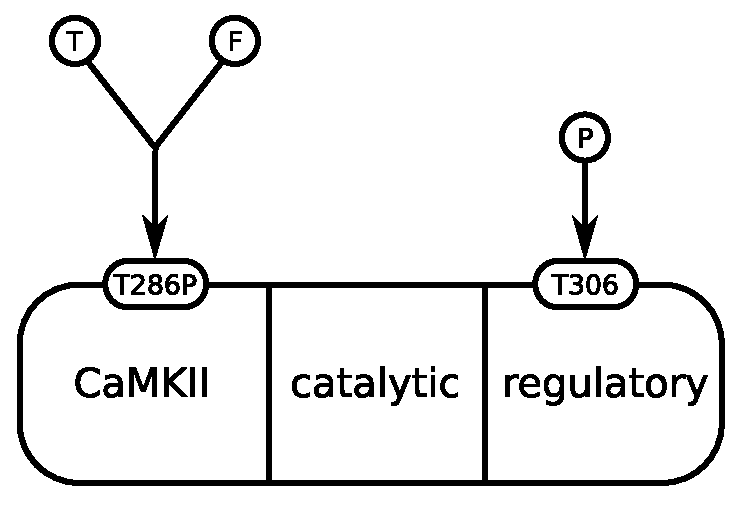
\includegraphics[scale = 0.5]{examples/ex-stateVariable}
  \caption{Two examples of \glyph{state variables} used to represent phophorylation of a threonine residue. While only the value ``phosphorylated'' is assigned to T306, the variable T286P can take the values true or false, which allow for representing dephosphorylation as well as phosphorylation.}
  \label{fig:ex-state-Variable}
\end{figure}

% \begin{figure}[H]
%   \centering
%   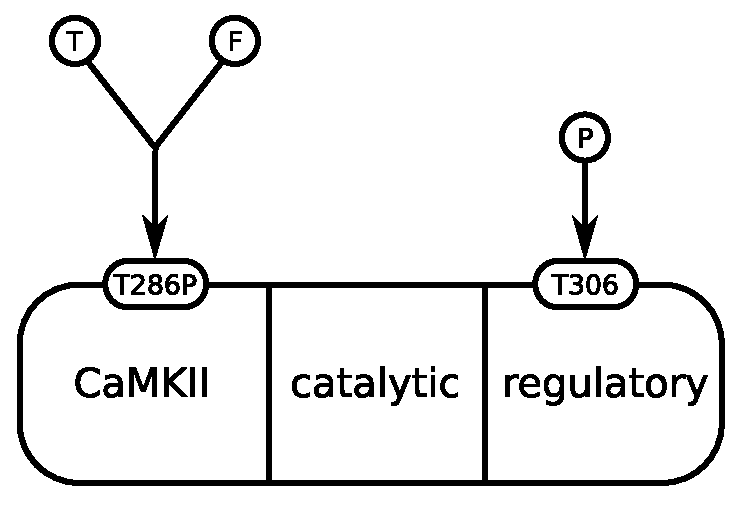
\includegraphics[scale = 0.5]{examples/ex-stateVariable}
%   \caption{Two examples of \glyph{state variables} used to represent phophorylation of a threonine residue. While only the value ``phosphorylated'' is assigned to T306, the variable T286P can take the values true or false, which allow for representing dephosphorylation as well as phosphorylation.}
%   \label{fig:ex-state-Variable}
% \end{figure}
% 
% Two state variables are predefined. The variable \glyph{existence} is used to represent the creation or destruction of entities, as seen on \fig{ex-existence}\label{sec:existence}. \glyph{Existence} can take two values, true (T) or false (F). The variable is represented by a circle vertically divided in two. One hemicircle is black, and the other white. 
% 
% \begin{figure}[H]
%   \centering
%   \includegraphics[scale = 0.5]{examples/ex-existence}
%   \caption{Using the \glyph{state variable} \glyph{existence} to represent the appearance of calcium following a depolarisation.}
%   \label{fig:ex-existence}
% \end{figure}
% 
% The variable \glyph{location} is used to represent the physical location of an entity, as seen on \fig{ex-location}\label{sec:location}. \glyph{Location} can take any value, but there can be only one \glyph{location} per entity. The variable is represented by a circle containing two perpendicular segments, an abstract version of the usual slanted pin.
% 
% \begin{figure}[H]
%   \centering
%   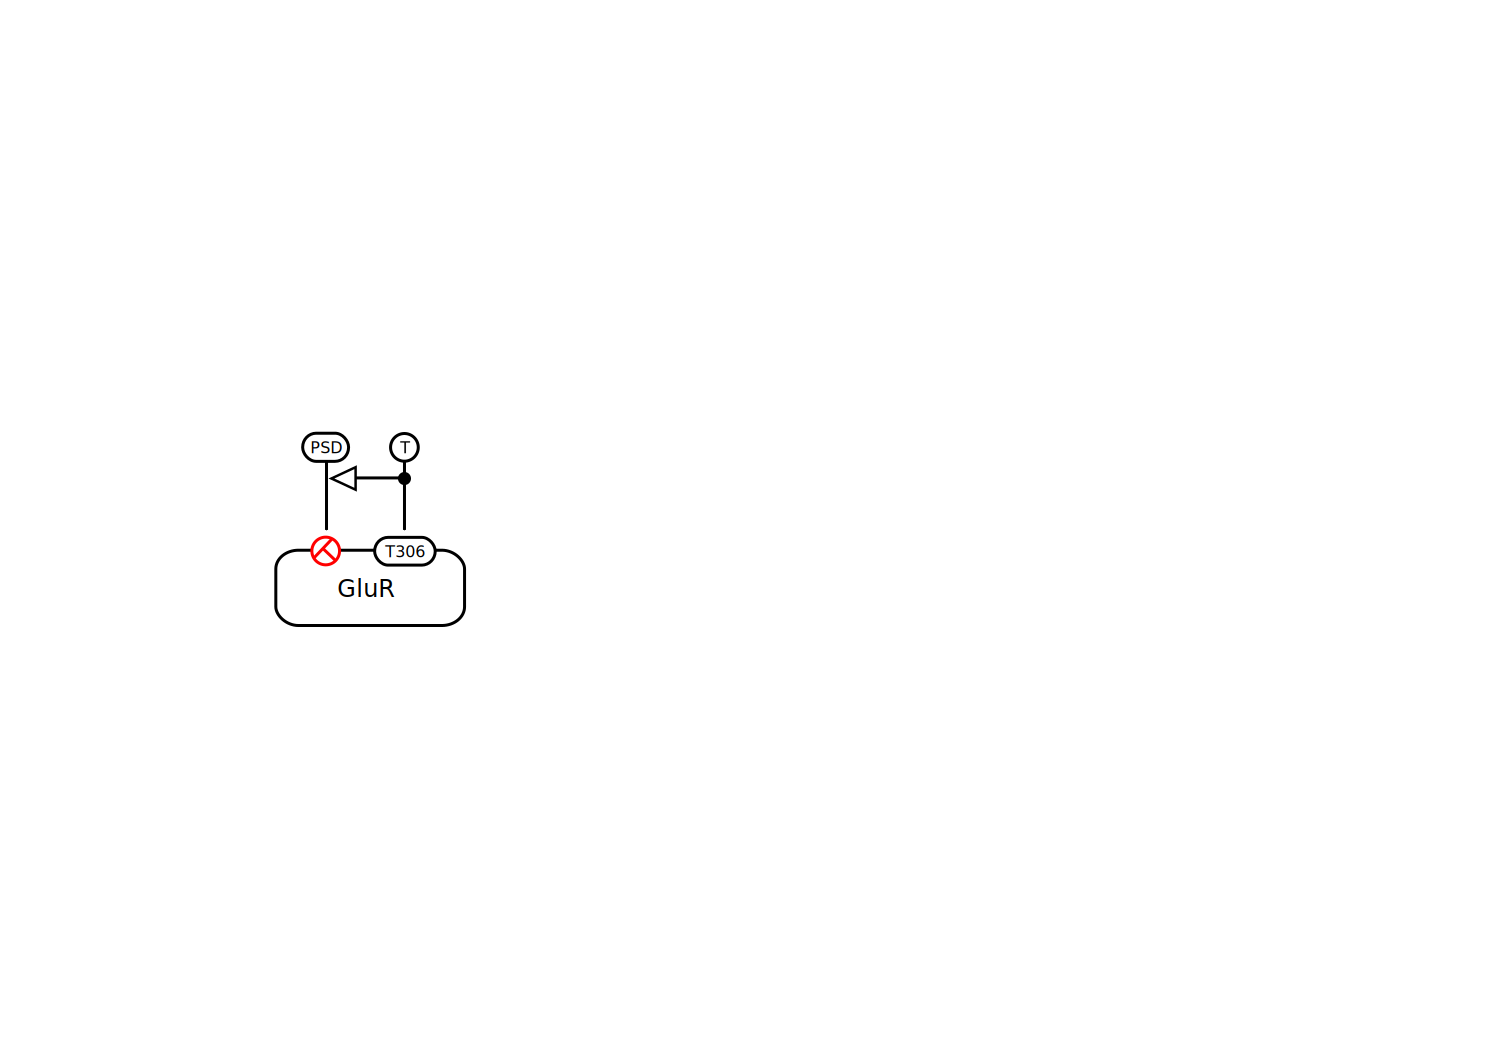
\includegraphics[scale = 0.5]{examples/ex-location-2}
%   \caption{Using the \glyph{state variable} \glyph{location} to represent the fact that phosphorylation of glutamate receptors stimulate their incorporation in the post-synaptic density.}
%   \label{fig:ex-location}
% \end{figure}

%\normalcolor

% The following is for [X]Emacs users.  Please leave in place.
% Local Variables:
% TeX-master: "../sbgn_ER-level1"
% End:

